\chapter{Boundary}

Architecture is defined by the boundaries drawn within a system and
the dependencies that cross those boundaries, rather than the physical
mechanisms through which components interact and execute functions..
Boundaries between components allow to make “firewalls” against
harmful propagation of changes.
The components on one side of the boundary change at different rates
and for different reasons than the components on the other side of the
boundary


\section{Drawing boundaries}

\begin{enumerate}
  \item Partition the system into components

  \item Identify core business components from those containing functions
        not related to the core business

  \item Arrange the code so that dependencies point toward the core
        business
\end{enumerate}

Make use of SOLID principles and Component principles.

\subsection{The clan architecture}

\begin{flushleft}
  \begin{minipage}{0.65\linewidth}
    \raggedright

    \begin{itemize}
      \item Outer circles: mechanisms.
      \item Inner circles: policies.
    \end{itemize}
    Dependency Rule : source
    code dependencies point
    only inward, toward inner
    circles (i.e. higher-level
    policies)

  \end{minipage}%
  \hfill
  \begin{minipage}{0.3\linewidth}
    \centering
    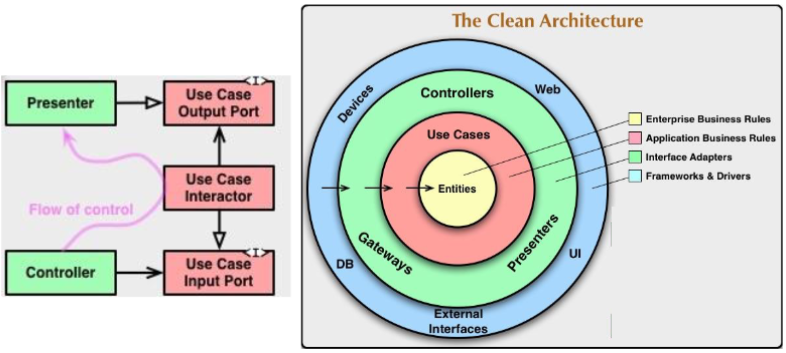
\includegraphics[width=\linewidth]{content/chapters/images/2026-05-05-18-04-48.png}
  \end{minipage}
\end{flushleft}

\subsection{Independence and Decoupling of layers}

Layers allow independent development, deployment, operation, and
maintenance.
Two type of layers: Horizontal (DB, UI, etc.) and Vertical (Source code units, services, etc.)



\begin{flushleft}
  \begin{minipage}{0.65\linewidth}
    \raggedright
    Decoupling of policy from the details.
    Defer decisions on details for as long as possible.

    DB component knows about use
    case rules component, but NOT
    viceversa. \textbf{Low level components know}
    everything of the \textbf{higher-level}
    components, but NOT viceversa.


    The Database
    component contains
    the code that translates
    the calls made by the
    BusinessRules into the
    query language of the
    database. This
    translation code knows
    about the
    BusinessRules.
    Business rules can be
    adapted to any kind of
    DB.

  \end{minipage}%
  \hfill
  \begin{minipage}{0.3\linewidth}
    \centering
    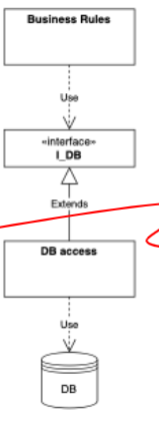
\includegraphics[width=0.3\linewidth]{content/chapters/images/2026-05-05-18-07-45.png}
  \end{minipage}
\end{flushleft}



\section{Crossing boundaries}

Are required for: require a service, ask for data or foward requests.
Only data cross boundaries, not entities. Data is passed in the most
convenient format for the inner circle.
Entity objects or database rows are NOT passed, otherwise Dependency
Rules mught be violated.

\paragraph{Low-level client to high-level server}

\begin{center}
  \begin{minipage}{0.65\linewidth}

    The Client calls a function
    f() on the Service. Data is passed as argument
    of the function.  Dependencies cross
    boundary from left to right
    point toward the higher-
    level component.
  \end{minipage}%
  \hfill
  \begin{minipage}{0.3\linewidth}
    \centering
    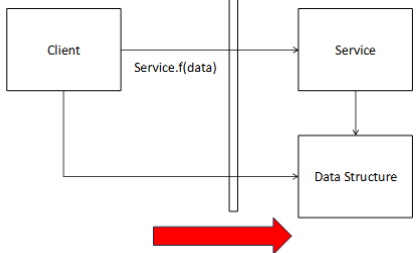
\includegraphics[width=0.6\linewidth]{content/chapters/images/2026-05-05-18-15-15.png}
  \end{minipage}
\end{center}


\paragraph{High-level client to low-level server}


\begin{center}
  \begin{minipage}{0.65\linewidth}
    The Client calls the f()
    function of the
    ServiceImpl, through
    the Service interface.
    Dependencies cross
    the boundary always
    toward the higher-
    level component.
  \end{minipage}%
  \hfill
  \begin{minipage}{0.3\linewidth}
    \centering
    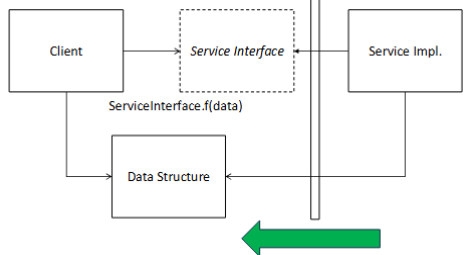
\includegraphics[width=0.6\linewidth]{content/chapters/images/2026-05-05-18-15-45.png}
  \end{minipage}
\end{center}

\subsection{Data is significant. Data storage is a detail}

From an architectural perspective, the database is NOT an entity.
It is a detail that does not rise to the level of an architectural element.

It is an architectural mistake to allow database rows and tables to be passed
around the system as objects. This is because it causes the use cases, business
rules and, in some cases, also the UI to be coupled to the relational structure
of the data.

The the data model, i.e. the organizational structure of data, instead,
is architecturally significant.

\paragraph{Example}

In our university, we need a software that manages the identities.
One of the use cases is to check identity from the polito badge and
grant/deny access for a specific area or room of the university.
It should be possible to check whether a person (student, professor, etc) have
access to a given laboratory in each department.

Policy about permissions (including which days and times, and for
how long time) are defined on a specific database.
Card readers use the magnetic stripe, but soon there will be also NFC
card readers in some department accesses.  A red or green light on the reader will show the result of the output


\subsubsection{Key aspects}


\begin{center}
  \begin{minipage}{0.75\linewidth}
    What is policy and what details ? Rreading bages, database, rules, output

    What is low level and what is high level ?

  \end{minipage}%
  \hfill
  \begin{minipage}{0.2\linewidth}
    \centering
    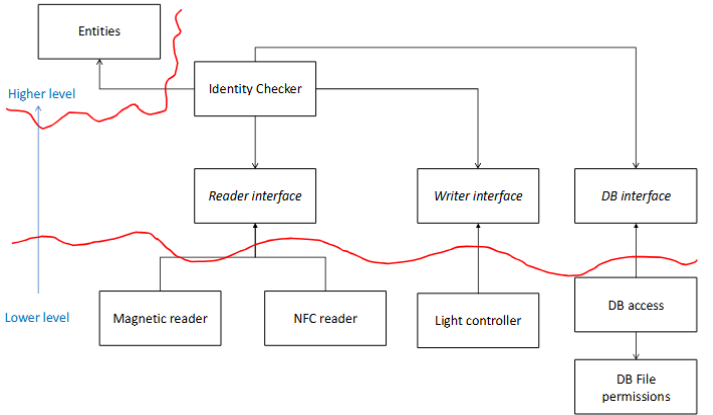
\includegraphics[width=\linewidth]{content/chapters/images/2026-05-05-18-25-00.png}
  \end{minipage}
\end{center}


\section{Layers}

The most basic components of a system are:
\begin{itemize}
  \item User Interface (UI)
  \item Application Logic
  \item Database
\end{itemize}

\paragraph{Example: a word processor}
A word processor (WP) is a device or software for creating, editing,
storing, and printing text documents.

\begin{figure}[h!]
  \centering
  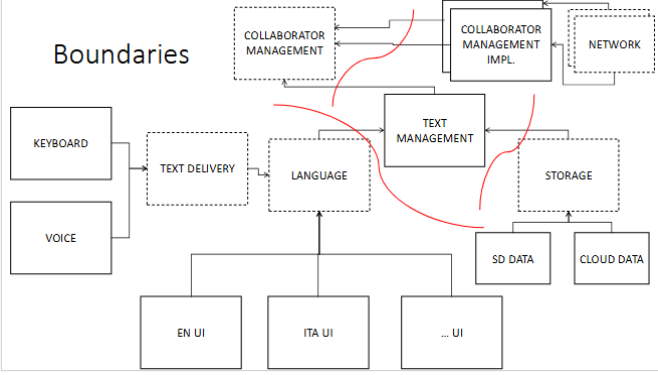
\includegraphics[width=0.4\linewidth]{content/chapters/images/2026-05-05-18-29-33.png}
\end{figure}

\section{Test}

Tests support development, not operation, HOWEVER
They are an integral component of the system, akin any other
elements within the system participate in its architecture.
They are part of the design of the system architecture.
Also tests adhere to the Dependency Rule.

\subsection{Design for testability}
Tests are coupled to other system's elements.
Changes to components in the inner circles may break several tests,
to reduce tests fragility, tests should depend as little as possible to
volatile elements.

Example: business rules should be tested without using the GUI.
Specific tests API can avoid constraints (e.g. security).

\subsection{Humble objects}

The Humble Object helps unit testers to separate behaviors that are
hard to test from behaviors that are easy to test.
It is adopted in software architecture to identify and protect
architectural boundaries.

\begin{figure}[h!]
  \centering
  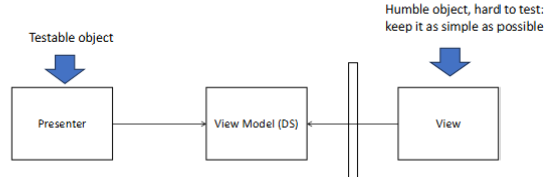
\includegraphics[width=0.4\linewidth]{content/chapters/images/2026-05-05-18-46-54.png}
\end{figure}
Esample are: Database gateways, Data mappers and Service listeners.


\section{Architectural styles}

Examples of SPG/order.

Use case: customers should be able to view the status of their orders

Classes:

\begin{itemize}
  \item OrdersController: web controller (e.g. Spring MVC controller) to handle requests from the web.
  \item OrdersService: interface that defines the logic related to orders.
  \item OrdersServiceImpl: The implementation of the orders service.
  \item OrdersRepository: An interface that defines how we get access to persistent order information
  \item JdbcOrdersRepository: An implementation of the repository interface.
\end{itemize}

option could be Package by layer or feature or component, Ports and Adapters

\begin{figure}[h!]
  \centering
  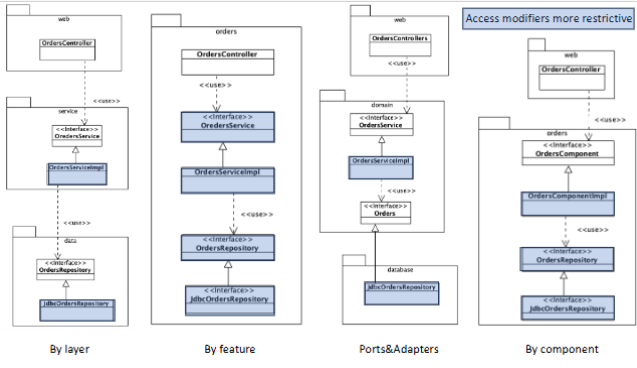
\includegraphics[width=0.5\linewidth]{content/chapters/images/2026-05-05-18-50-31.png}
\end{figure}

\subsection{Package by layer}

Code is organized into layers
according to its behavior. Each layer depends only on the
next adjacent lower layer. E.g.: webcode, business logic,
persistence

\begin{itemize}
  \item \textbf{Pros:} simple, Tied to technical view, Commonly used
  \item \textbf{Cons:} As software grows, layers become “fat”, It is not tied to a the specific “business”
        view (the same for any domain). Dependencies are still possible between
        not adjacent layers
\end{itemize}


\subsection{Package by feature}

Vertical slicing by feature


\begin{itemize}
  \item \textbf{Pros:} It well reflects the domain, Everything about a functionality is
        in one package
  \item \textbf{Cons:} Suboptimal in terms of separation
        of implementation details and
        business logic
\end{itemize}


\subsection{Ports and Adapters}

Domain-specific code (inner circle)
is well separated from
implementation details (outer
circles). The latter depends on the former:
the dependencies flow from
outside toward inside.


\subsection{Package by component}
Service-centric view.
Everything needed for orders is in
the OrdersComponent. Separation of concerns is
maintained inside each compone


\section{Architectural styles}
Reusable set of structural principles and high-level design decisions on:

\begin{itemize}
  \item Component topology: by technical capabilities/by domain
  \item Physical architecture: monolithic/distributed
  \item Deployment: system's granularity and deployment frequency
  \item Communication style: synchronous/asynchronous, protocols/calls/queues
  \item Data topology: monolithic database/separate data
  \item Team topologies: remember Conway's law
\end{itemize}

\textbf{Monolithic} = single deployment unit of all code

\textbf{Distributed} = multiple deployment units connected through remote
access protocols

\begin{figure}[h!]
  \centering
  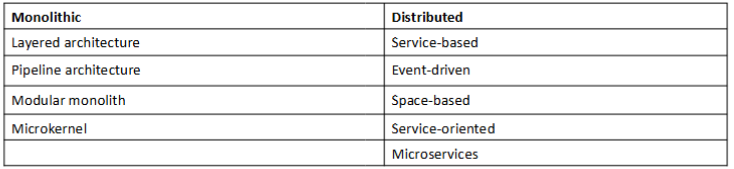
\includegraphics[width=0.5\linewidth]{content/chapters/images/2026-05-05-18-55-22.png}
\end{figure}















